\documentclass[a4paper,10pt]{article}
\usepackage{graphicx}
\usepackage{float}
\usepackage{booktabs}
\usepackage{amsmath}
\usepackage{amssymb}
\usepackage{amsthm}
\usepackage{physics}
\usepackage{geometry}

\newcommand*{\unit}[1]{\ensuremath{\mathrm{\,#1}}}

\title{High-Purity germanium detectors}
\author{Gianluca Cavallaro \\ Marco Gobbo}
\date{20 Aprile 2020}
\begin{document}
\maketitle
\section{Introduzione}
La seguente esperienza ha come scopo quello di studiare la caratterizzazione di due diversi rivelatori al germanio. Per avere un quadro più completo, illustriamo brevemente le caratteristiche di questi tipi di rivelatori. Si tratta di una classe di rivelatori a semiconduttore, il germanio in questo caso, che sfrutta la tecnologia della giunzione P-N. La giunzione P-N è costituita da due zone, una con un eccesso di lacune ed una con un eccesso di elettroni. Lacune ed elettroni vengono ottenuti mediante diverse tecniche di drogaggio del materiale utilizzato. La zona chiave della giunzione P-N è quella di confine tra le due zone: i portatori di carica possono diffondere nella zona adiacente, attraverso una corrente di diffusione, creando, in ultima istanza, una differenza di potenziale che genera un campo elettrico, che a sua volta genera una corrente di trascinamente che si oppone a quella di diffusione. Le caratteristiche delle due zone e dei portatori di carica dipende dalle caratteristiche costitutive della giunzione. La giunzione può poi essere sottoposta a polarizzazione diretta o inversa: nel nostro caso siamo interessati a polarizzare inversamente la giunzione, cosi che nel nostro rivelatore non ci sia nessuna corrente sovrapposta a quella di raccolta delle cariche. Il rivelatore va poi tenuto in un dewar che lo mantiene ad una temperatura di 77K, attraverso un bagno di azoto liquido. Questo perchè nei semiconduttori la banda di valenza e di conduzione è separata da un gap in energia, che nel germanio è talmente basso (0.67 eV) che mantenendo il rivelatore a temperatura ambiente l'agitazione termica sarebbe sufficiente a superare questo gap, ostacolando le nostre misure.
\section{Parte 1}
\subsection{Strumentazione}
\begin{itemize}
\item Crate NIM per alimentazione di elettronica standard
\item Rivelatore coassiale HPGe 
\item Generatore HV Label Model 8124 per tensione di polarizzazione
\item Amplificatore CAEN Model N968
\item ADC/MCA CAEN Model N957
\item Sorgenti di calibrazione: 22Na, 60Co, 228Th
\end{itemize}
\subsection{Scelta delle condizione ottimali di lavoro}
Il segnale è acquisito mediante una catena di lettura classica. In questo caso abbiamo un dispositivo che integra detector e pre-amplificatore, uno che integra amplificatore e shaper e un ADC/MCA a parte. L'obiettivo di questa prima parte è quello di individuare le condizioni ottimali per tensione di polarizzazione e shaping time per proseguire nell'esperienza. Individuare le condizioni di lavoro ottimali significa individuare quelle che minimizzano la risoluzione. Abbiamo a nostra disposizione degli spettri di una sorgente di 22Na, raccolti in corrispondenza di diversi valori di polarizzazione, da 2000V a 5000V, e di shaping time, rispettivamente 0.5, 1, 2, 3, 6, e 10 $\mu$s. 

\begin{figure}[h!]
    \centering
    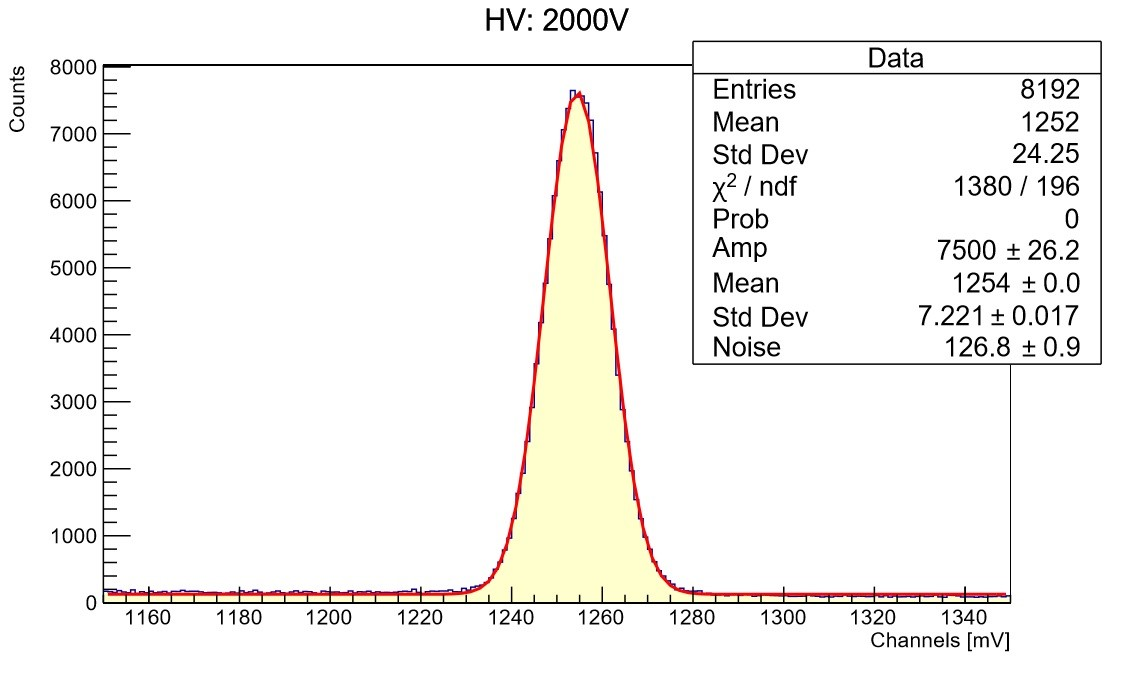
\includegraphics[scale=0.45]{grafici/hv}
    \caption{Tensione di polarizzazione 2000V}
\end{figure}

\begin{figure}[h!]
    \centering
    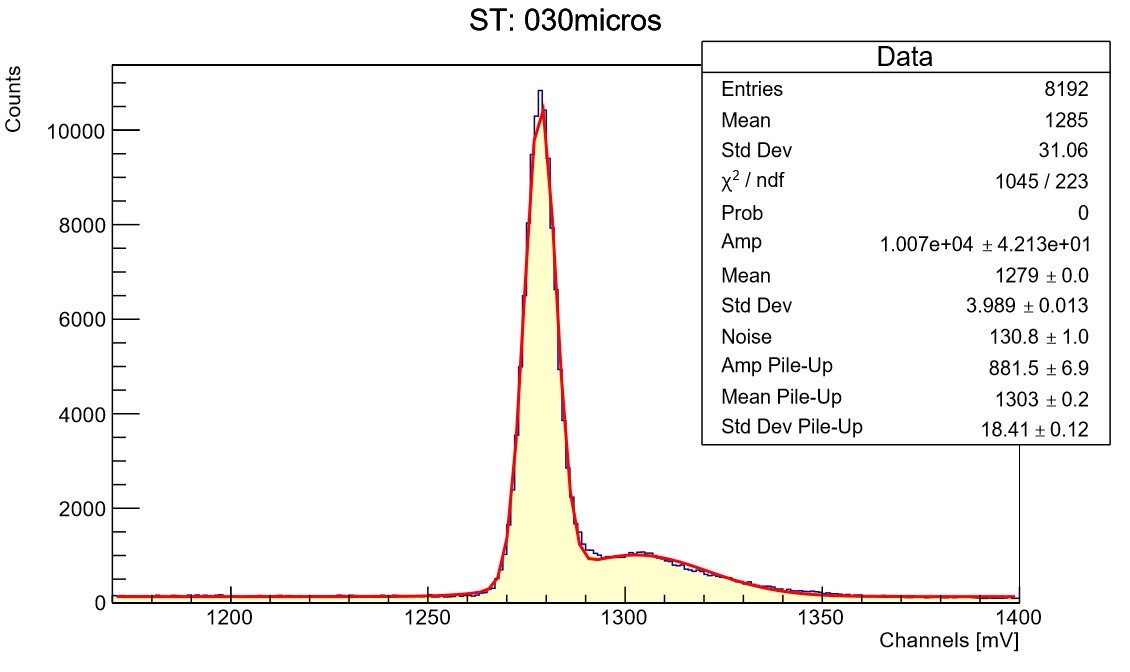
\includegraphics[scale=0.45]{grafici/st}
    \caption{Shaping time 30 $\mu$s}
\end{figure}

Per i grafici relativi alla tensione di polarizzazione è stato necessario effettuare uno "zoom" sulla zona dove si registra il picco. In questa zona, il picco è stato estrapolato attraverso una funzione gaussiana sommata ad un polinomio di grado 0, che tiene conto del fondo. Nei grafici relativi allo shaping time il procedimento è stato analogo, ma nel fittare la funzione è stato necessario considerare due gaussiane, con la seconda che ci ha permesso di considerare nel fit il pile-up, fenomeno per il quale il rivelatore non è "pronto" a ricevere due misure successive, e va quindi a sommare un evento sulla coda di quello precedente, andando in alcuni casi a deformare il picco in questione. Attraverso questo processo siamo arrivati ad avere a disposizione 16 valori per la tensione di polarizzazione e 6 per lo shaping time. Per entrambe le raccolte dati, andiamo a costruire il grafico della risoluzione in funzione della tensione di polarizzazione e dello shaping time, rispettivamente. La risoluzione è stata calcolata con la seguente relazione: 

\begin{equation}
	R=\frac{\textrm{FWHM}}{\textrm{Channel}}
\end{equation}

\begin{figure}[h!]
    \centering
    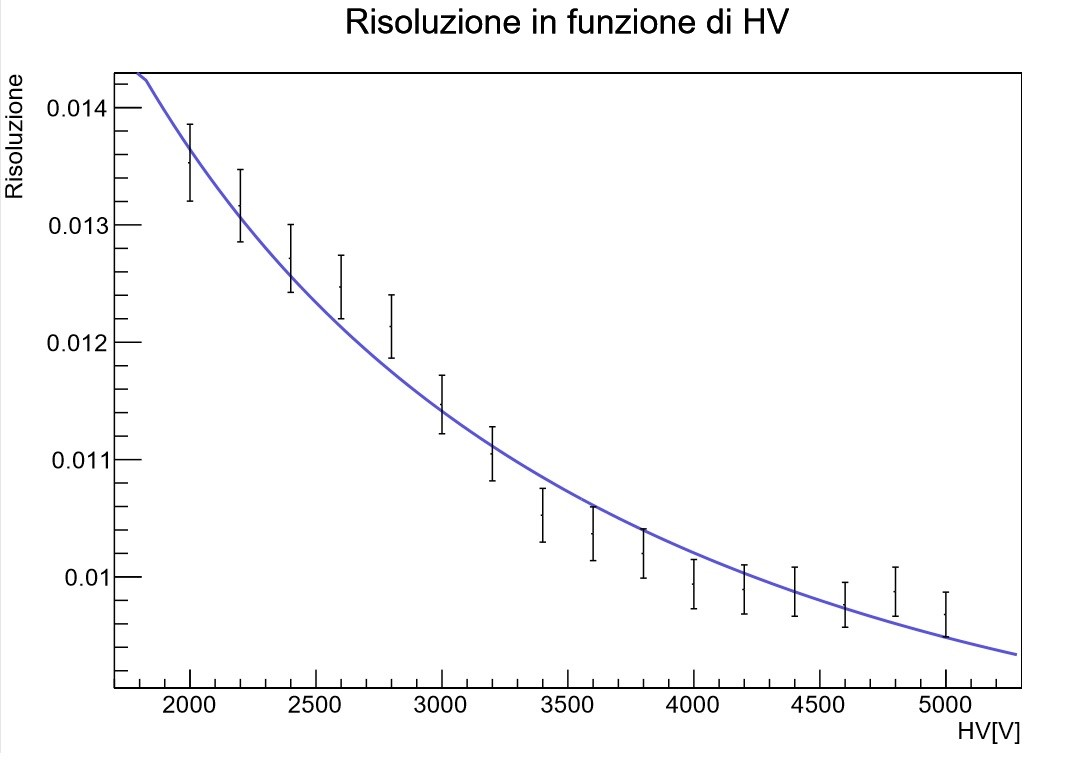
\includegraphics[scale=0.45]{grafici/risoluzionehv}
    \caption{Risoluzione in funzione della tensione di polarizzazione}
\end{figure}

-inserire grafico risoluzione st-

I grafici sono stati interpolati con la seguente funzione: 
\begin{equation}
	R=\sqrt{\frac{\textrm{a}}{\textrm{x}}+\textrm{bx}}
\end{equation}
con x che indica in un caso la tensione e nell'altro lo shaping time.

Il nostro obiettivo era di ricavare i valori che minimizzassero la risoluzione. Nel caso della tensione di polarizzazione la risoluzione decresce, fino ad assestarsi intorno ad un valore costante oltre i 4000V, che può quindi essere preso come valore di riferimento. Nel caso dello shaping time la risoluzione ha un minimo in corrispondenza di uno shaping time di 2 $\mu$s, ed oltre quel valore torna a crescere, a causa del pile-up che diventa sempre più significativo.
\subsection{Calibrazione in energia del rivelatore}
\subsubsection{Curva di calibrazione}
Abbiamo a disposizione gli spettri di 3 sorgenti note: 22Na, 60Co e 228Th. Gli spettri sono riportati in appendice. Come fatto precedentemente, andiamo ad effettuare uno "zoom" su ognuno dei picchi per poterne ottenere la posizione e la sigma. Per il torio in particolar modo, abbiamo tenuto conto solo dei picchi più intensi e distinguibili. Di seguito riportiamo un esempio:

\begin{figure}[h!]
    \centering
    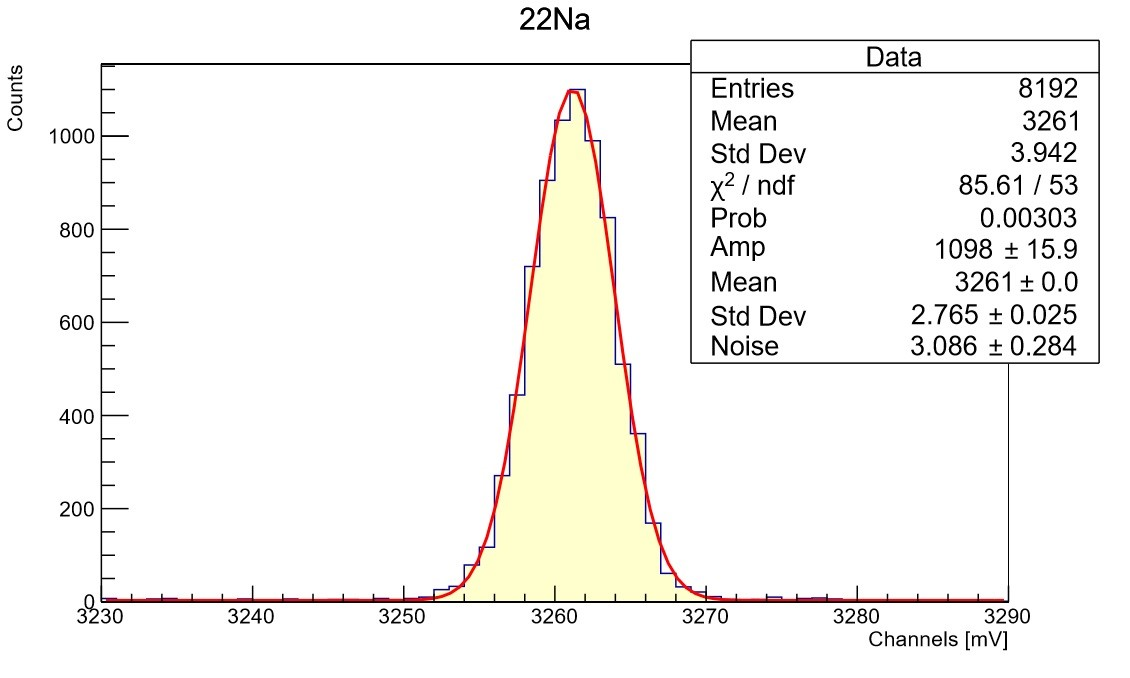
\includegraphics[scale=0.45]{grafici/piccoNa}
    \caption{Il picco del 22Na}
\end{figure}

\begin{figure}[h!]
    \centering
    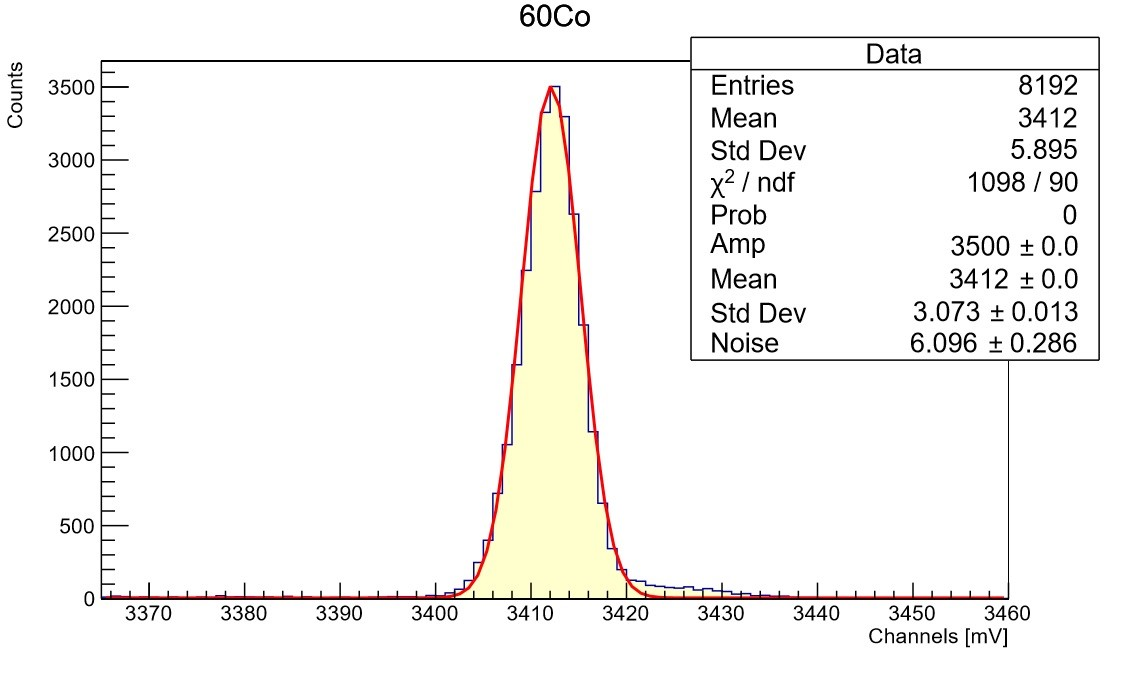
\includegraphics[scale=0.45]{grafici/piccoCo}
    \caption{Uno dei due picchi del 60Co}
\end{figure}

\begin{figure}[h!]
    \centering
    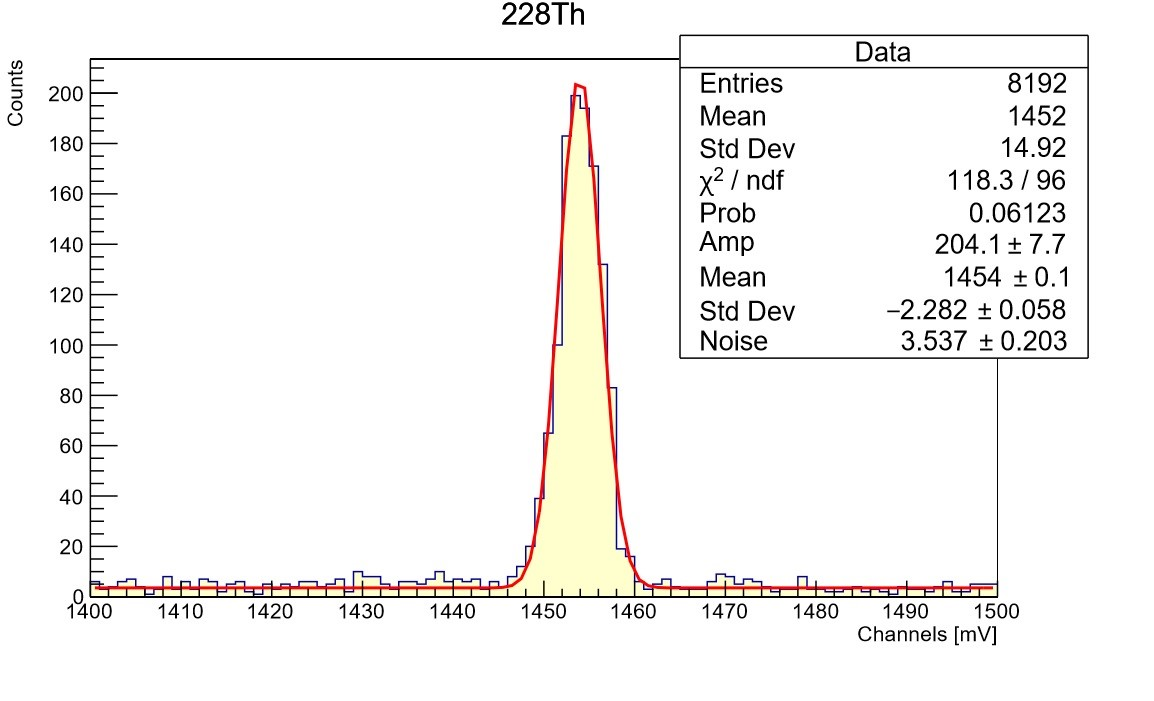
\includegraphics[scale=0.45]{grafici/piccoTh}
    \caption{Uno dei picchi del 228Th}
\end{figure}

Ognuno dei picchi individuati corrisponde ad una energia ben precisa. Nel seguente grafico è dunque riportata la curva di calibrazione, Energia vs. Canali:

\begin{figure}[H]
    \centering
    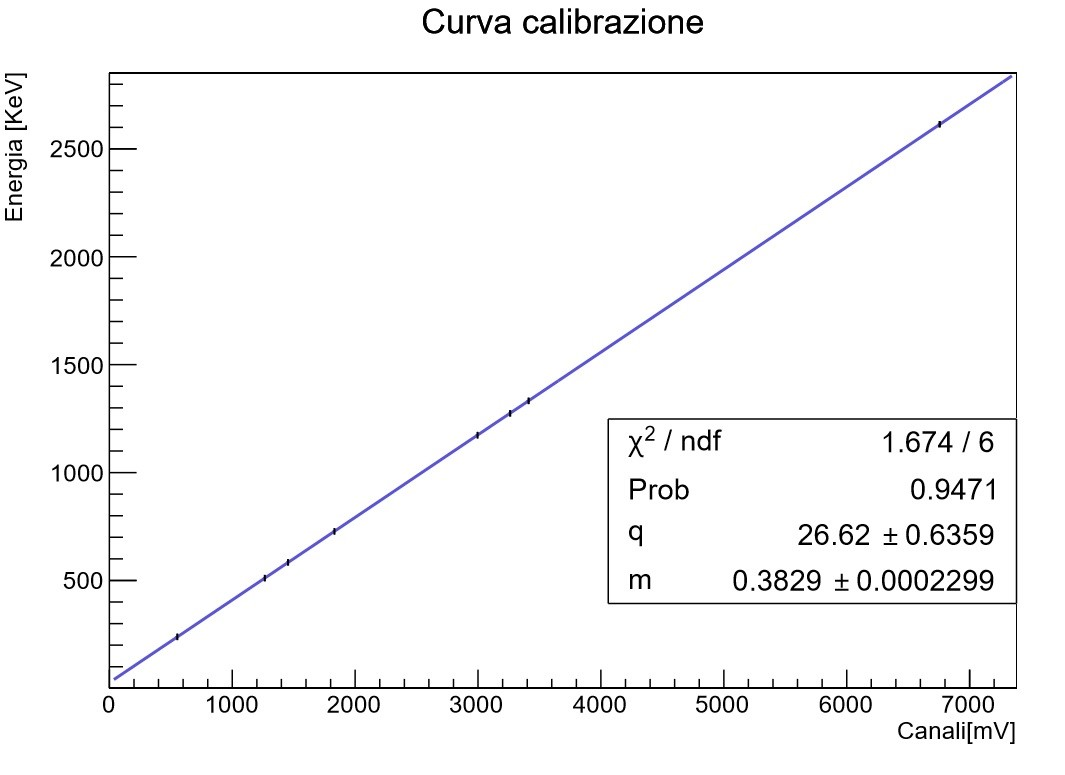
\includegraphics[scale=0.45]{grafici/rettacalibrazionesources}
    \caption{Energia vs. Canali}
\end{figure}

Il grafico è stato interpolato con la seguente funzione 
\begin{equation}
	Energia=m\cdot Canale + q
\end{equation}

ottenendo i seguenti parametri:

$$
	m=0.3829 \pm 2.3 \times 10^{-4}\, \unit{Kev/V}
$$
$$
	q=26.62 \pm 0.64\, \unit{Kev}
$$

I valori di $\chi$\textsuperscript{2} ridotto e \textit{P-Value} riportati nel grafico mostrano come l'andamento lineare della relazione sia consistente. La relazione che intercorre fra energia e canali è dunque lineare.

\subsubsection{Risoluzione}
Vogliamo andare ad indagare la dipendenza della risoluzione in funzione dei valori di energia. La risoluzione è caratterizzata da 3 componenti: una statistica, che dipende linearmente dall'energia, una legata alla raccolta delle cariche, che dipende quadraticamente dall'energia, ed infine una legata al rumore elettronico, indipendente dall'energia. La risoluzione è stata calcolata con la relazione (1). Per quanto riguarda le incertezza si è tenuto conto della deviazione standard e dell'errore su quest'ultima. 

\begin{figure}[H]
    \centering
    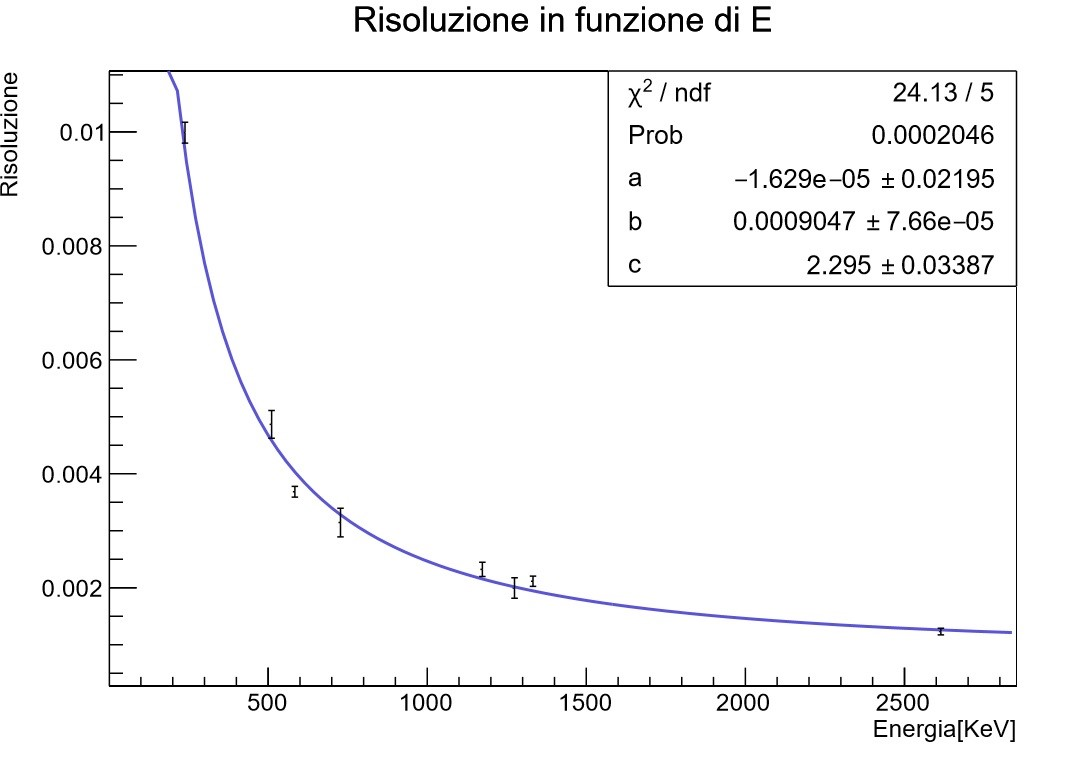
\includegraphics[scale=0.45]{grafici/risoluzionesources}
    \caption{Risoluzione in funzione di E}
\end{figure}

Per interpolare il grafico è stata utilizzata la relazione

\begin{equation}
	R=\sqrt{\frac{a^2}{E}+b^2+\frac{c^2}{E^2}}
\end{equation}

Con a, b e c che rispettivamente indicano i contributi legati alla statistica, alla raccolta delle cariche e al rumore. Sono riportati di seguito i valori:

$$
	a=1.63 \times 10{-5} \pm 2.20 \times 10^{-2}
$$
$$
	b=9.01 \times 10^{-4} \pm 7.66 \times 10{-5}
$$
$$
	c= 2.29 \pm 3.38 \times 10^{-2}
$$

Da cui risulta evidente che il contributo principale alla risoluzione sia legato al rumore elettronico.

\end{document}